
\section{First section}
Existing surface integration methods for range images can be classified into two categories: volume-based and mesh-based. Volume-based methods \cite{Claes:VolM05,Curless:VolM96,Masuda:VolM02,Hoppe:VolM97,Sato:VolM97,Sun:VolM03} convert range images into an intermediate volumetric representation using a signed distance function and extract the final surface using a polygonizing algorithm. These methods can handle objects of arbitrary topology and are considered to be robust with respect to scanning noise, outliers and registration errors. The choice of appropriate voxel size is important for these methods \cite{Claes:VolM05,Curless:VolM96}. If the voxel size is too large, then features smaller than the voxel size are missed and opposite surfaces of a narrow region will be merged. If the voxel size is too small, then in the presence of scanning noise or registration errors, corresponding surfaces will be reconstructed as separate surfaces. It still remains unanswered as to what extent the signed distance function computed on the discretized space is sensitive to the presence of noisy data. It is also not clear how to choose an appropriate voxel size when the input range images have both small features and registration errors. \\

Mesh-based methods \cite{Pito:MeshM96,Rutishauser:MeshM94,Sappa:MeshM00,Soucy:MeshM92,Soucy:MeshM95,Sun:MeshM00,Turk:MeshM94,Zhou:MeshM06} directly integrate range images into a single mesh. These methods do not need an intermediate representation. Hence, they are faster and require less memory compared to volumetric methods. In addition, they are more amenable to data reduction during processing which makes them more feasible for use with very large meshes. Existing methods are, however, sensitive to scanning errors and do not work well on objects with large surface curvature \cite{Curless:VolM96}.

\begin{figure}[t]
    \centering
    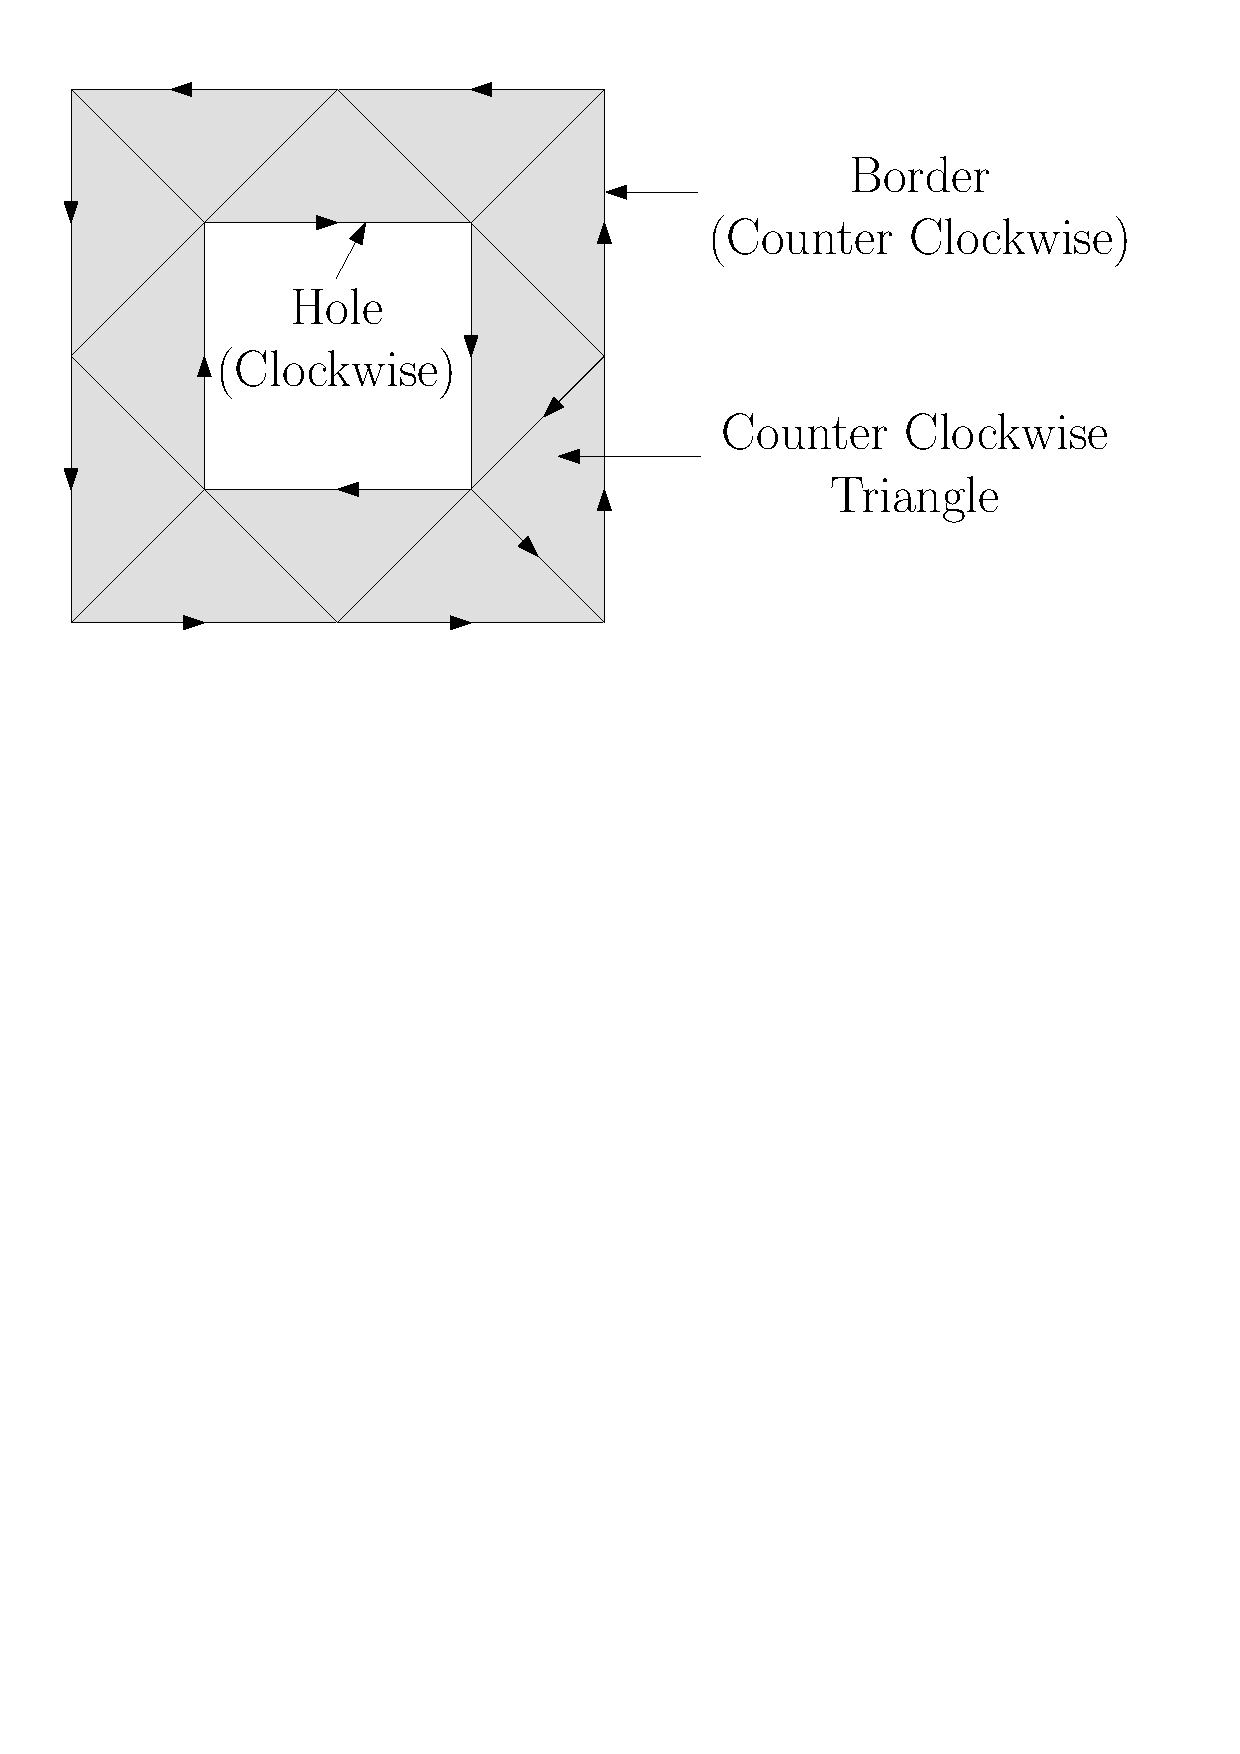
\includegraphics[width=5in]{border}
    \caption[Boundary edges]{Boundary edges.}
    \label{fig:Ch1-border}
\end{figure}
\input{table}

